This chapter presents examples of \abcpt{}s created using \abcdt{}, thus demonstrating how easily a
(simple) tool or some occasional processing can be done. Some of the tools presented are an
extension of those presented in the article~\cite{Azevedo2013} submitted and accepted to
\emph{SLATE'13}'s conference.

The tools presented here are merely a proof of concept of what can be done with \abcdt{}, therefore,
they only provide a limited number of features and can be further improved in the future. However,
as they are, some of them have already proven their worth, consult chapter
\ref{chap:test_eval}.

Every \abcpt{} created performs at least one traversal to an \abc{} \ac{IR} (through \dt{}). So, in
order to facilitate the \abcdtrules{} readability for each \dt{} call, a tabular format will be
used, in which each row describes a single \abcdtrule{}.

%TODO nas regras (tabelas) por codigo perl mais bonito (fancy verbatim) ou letra mais pequena
%todo SE TIVER tempo por attach (midi)

\section{Paste ABC}
This tool, as the \unix{} \emph{paste}, merges voices parallel to each other in the time
perspective. In other words, each individual voice will start at the beginning of the resulting
score.

Some decisions were made regarding what should be done with some information present in each tune.
This ensured that the resulting tune was consistent with each individual tune:

\begin{enumerate}
  \item The resulting tune's header derives from the first tune which has an actual tune written, in
  other words, at least one \emph{note}.
  \item The \context{} is updated every time a change is detected during the tune's traversal. It is
  a local data structure that comprises the \emph{current voice} and its \emph{key}, \emph{meter},
  \emph{length}, \emph{tempo} and \emph{number of measures}.
  \item Any \context{} change detected, like the \emph{key} or the \emph{meter}, is written to the
  resulting tune only if it is different from the current \context{}.
  \item In the resulting tune, any voice that has fewer measures than the longest one is appended
  with the necessary \measurerests{} to match the longest.
\end{enumerate}

\subsection*{Algorithm}

\pasteabc{}'s algorithm is divided in three stages: \textbf{1)} retrieving the header for the
resulting tune, \textbf{2)} pasting the tunes and \textbf{3)} appending any necessary
\measurerests{}. In the end, the output generated is printed to the output.

An algorithmic description is made in algorithm \ref{alg:pasteabc}.

\begin{enumerate}
\item As mentioned before, the resulting tune's header comes from the first tune with at least
one \emph{note} written.

This stage follows a simple algorithm where each tune is processed by \dt{} in the order they are
passed in. As soon as a tune with a \emph{note} written is found, it stops and returns that tune's
header. During the tune's traversal, the \context{} is updated. It will be used in the final stage
where a post processing is done to guarantee the resulting tune's validity.

The set of \abcdtrules{} to be passed to \dt{} consists in applying a blank transformation to every
\abcelement{} with state \intune{} or \inline{} (consult section \ref{sec:abcdt_rules} for more
information on state), activating a flag when a \emph{note} is found to stop processing further
tunes and, finally, recording the \context{}. See table \ref{tab:paste_fst_stg_rules} for a
description of the \abcdtrules{}.

\begin{center}
  \begin{table}[h]
    \begin{tabular}{|p{2.25cm}|p{7.25cm}|p{5cm}|}
      \hline
      Actuator & Transformation (Perl) & Notes\\
      \hline
      \hline
      \intune{} & q\{\}; &
      \\
      \hline

      \hline
      \inline{} & q\{\}; &
      \\
      \hline

      \hline
      \emph{note} & \$has\_tune = 1; q\{\}; &
      \\
      \hline

      \hline
      \inheader{}::\emph{M:} & update\_context(\{meter => 1\}); toabc(); & \emph{update\_context} is
      a local function that updates, in this rule's case, the \context{}'s meter. \toabc{} is called
      in the end so that the actual \abcelement{} is printed instead of the returning value from the
      previous statement.
      \\
      \hline

      \hline
      \inheader{}::\emph{L:} & update\_context(\{length => 1\}); toabc(); &
      \\
      \hline

      \hline
      \inheader{}::\emph{K:} & update\_context(\{key => 1\}); toabc(); &
      \\
      \hline

      \hline
      \inheader{}::\emph{Q:} & update\_context(\{tempo => 1\}); toabc(); &
      \\
      \hline
    \end{tabular}
    \caption{\abcdtrules{} for \pasteabc{}'s first stage}
    \label{tab:paste_fst_stg_rules}
  \end{table}
\end{center}

\item This stage's consists in processing each tune with \dt{} and concatenating each individual
result. This is the actual pasting where each tune's original \abc{} is returned except for the
following parts.

The header from each tune is not printed since it has already been retrieved in the previous stage.

abcMIDI commands \emph{\%\%staves} and \emph{\%\%score} are not printed as well, since each voice's
positioning on the resulting score may differ from the original one.

The \context{} is also being recorded each time one of its constituents is found, which enables the
possibility of not printing the context change if it is the same as the current one. This makes the
resulting tune cleaner without useless duplications. See table \ref{tab:paste_snd_stg_rules}.

\begin{center}
  \begin{table}[h]
    \begin{tabular}{|p{2.5cm}|p{4.75cm}|p{8cm}|}
      \hline
      Actuator & Transformation (Perl) & Notes\\
      \hline
      \hline
      \emph{in\_global::info} & q\{\}; &
      \\
      \hline

      \hline
      \emph{in\_header::info} & q\{\}; &
      \\
      \hline

      \hline
      \emph{staves} & q\{\}; &
      \\
      \hline

      \hline
      \emph{score} & q\{\}; &
      \\
      \hline

      \hline
      \emph{bar} & update\_measure\_count(); toabc(); & \emph{update\_measure\_count} is a local
      function that increments the measure count for the current voice.
      \\
      \hline

      \hline
      \emph{V:} & print\_voice(); & Local function that prints the voice element if it is different
      from the current voice. Also, if this voice has been previously defined, then the short form
      of the voice's \abcelement{} is printed. \context{}'s voice is updated.
      \\
      \hline

      \hline
      \emph{M:} & print\_meter(); & Local function that prints the meter element if it is different
      from the current meter. \context{}'s meter is updated.
      \\
      \hline

      \hline
      \emph{L:} & print\_length(); & Same as the previous rule but applied to the length element.
      \\
      \hline

      \hline
      \emph{K:} & print\_key(); & Same as the previous rule but applied to the key element.
      \\
      \hline

      \hline
      \emph{Q:} & print\_tempo(); & Same as the previous rule but applied to the tempo element.
      \\
      \hline

    \end{tabular}
    \caption{\abcdtrules{} for \pasteabc{}'s second stage}
    \label{tab:paste_snd_stg_rules}
  \end{table}
\end{center}

\item The final step consists in verifying if there is any voice with fewer measures than the voice
with the biggest number of measures. If there is such a voice then a \measurerest{} with length
equal to the missing measures is appended after that voice. This is possible because, in step
\textbf{2)}, the number of measures for each voice was being recorded.
\end{enumerate}

\begin{algorithm}[h]
  \KwIn{abc\_tunes}
  \ForAll{$ tune \in abc\_tunes $}{
    $header \gets dt(tune,$ rules from table \ref{tab:paste_fst_stg_rules}$)$ \hfill //1)\\
  }
  \ForAll{$ tune \in abc\_tunes $}{
    $res \gets res$ ++ $dt(tune,$ rules from table \ref{tab:paste_snd_stg_rules}$)$ \hfill //2)\\
  }
  $measures \gets add\_measures()$ \hfill //3)\\
  \Return{$header$ ++ $res$ ++ $measures$}
  \caption{\pasteabc{}'s algorithm}
  \label{alg:pasteabc}
\end{algorithm}

\subsection*{Usage}

Listing \ref{lst:pasteabcman} shows \pasteabc{}'s manual.\\

\lstinputlisting[caption={\pasteabc{}'s manual},label={lst:pasteabcman},captionpos=t,abovecaptionskip=-\medskipamount,float]{misc/paste_manual.tex}

Listing \ref{lst:paste_abc_by_example} shows a usage example for \pasteabc{}. It reads tunes
\textbf{101.abc} (listing \ref{lst:verbum_s1_p1}) and \textbf{103.abc} (listing
\ref{lst:verbum_s1_p3}) and its output is shown in listing \ref{lst:verbum_s1_p1_p3_pasted} along
with the corresponding score (figure \ref{fig:verbum_s1_p1_p3_score}).\\

\begin{lstlisting}[caption={\pasteabc{} by example},label={lst:paste_abc_by_example},captionpos=t,abovecaptionskip=-\medskipamount]
paste_abc 101.abc 103.abc
\end{lstlisting}

\lstinputlisting[caption={Verbum caro factum est: Section 1; Part 1 - Soprano},label={lst:verbum_s1_p1},captionpos=t,abovecaptionskip=-\medskipamount]{misc/verbum_s1_p1.tex}

\vspace{-0.25cm}
\begin{figure}[H]
  \begin{center}
    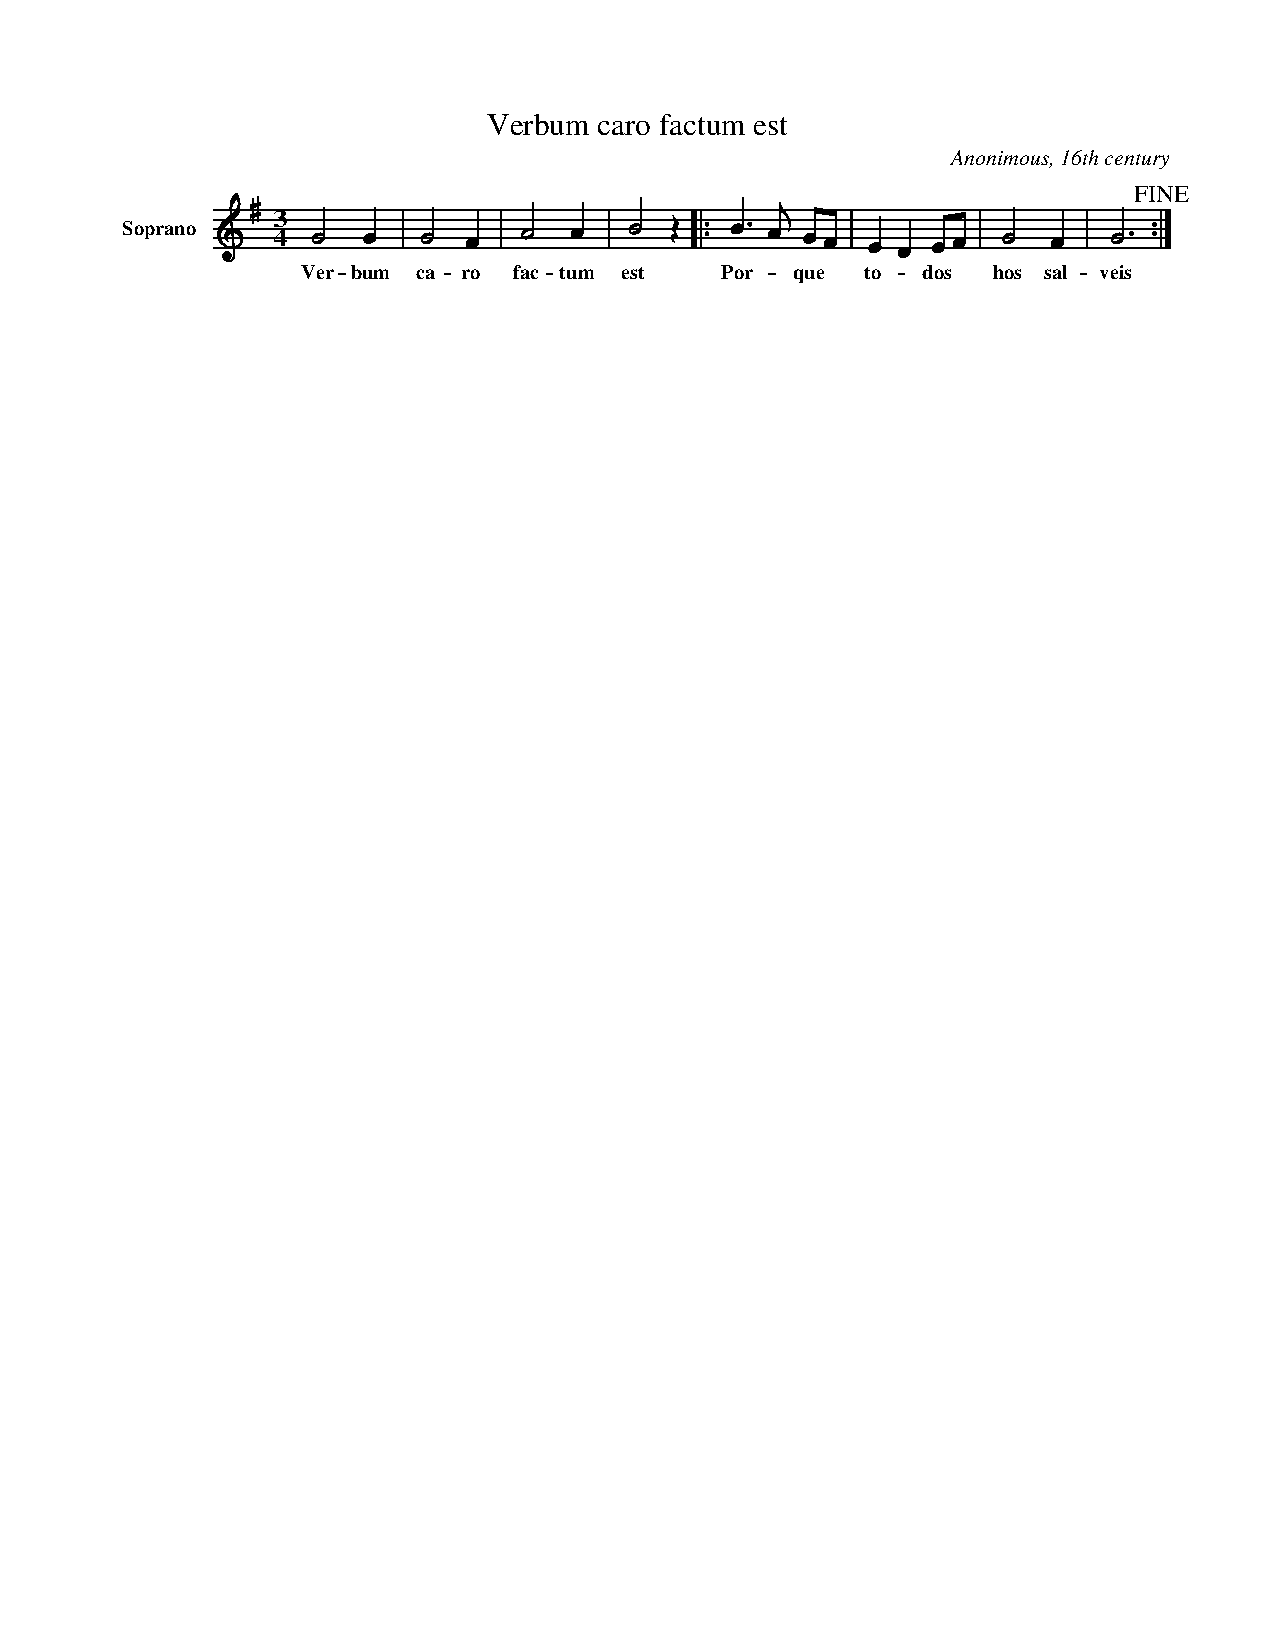
\includegraphics[width=0.8\textwidth, clip=true, trim = 0mm 230mm 0mm 17mm]{img/101.pdf}
    \caption{Verbum caro factum est: Section 1; Part 1 - Soprano (Score)}
    \label{fig:verbum_s1_p1_score}
  \end{center}
\end{figure}

\lstinputlisting[caption={Verbum caro factum est: Section 1; Part 3 - Tenor},label={lst:verbum_s1_p3},captionpos=t,abovecaptionskip=-\medskipamount]{misc/103.tex}

\vspace{-1.30cm}
\begin{figure}[h]
  \begin{center}
    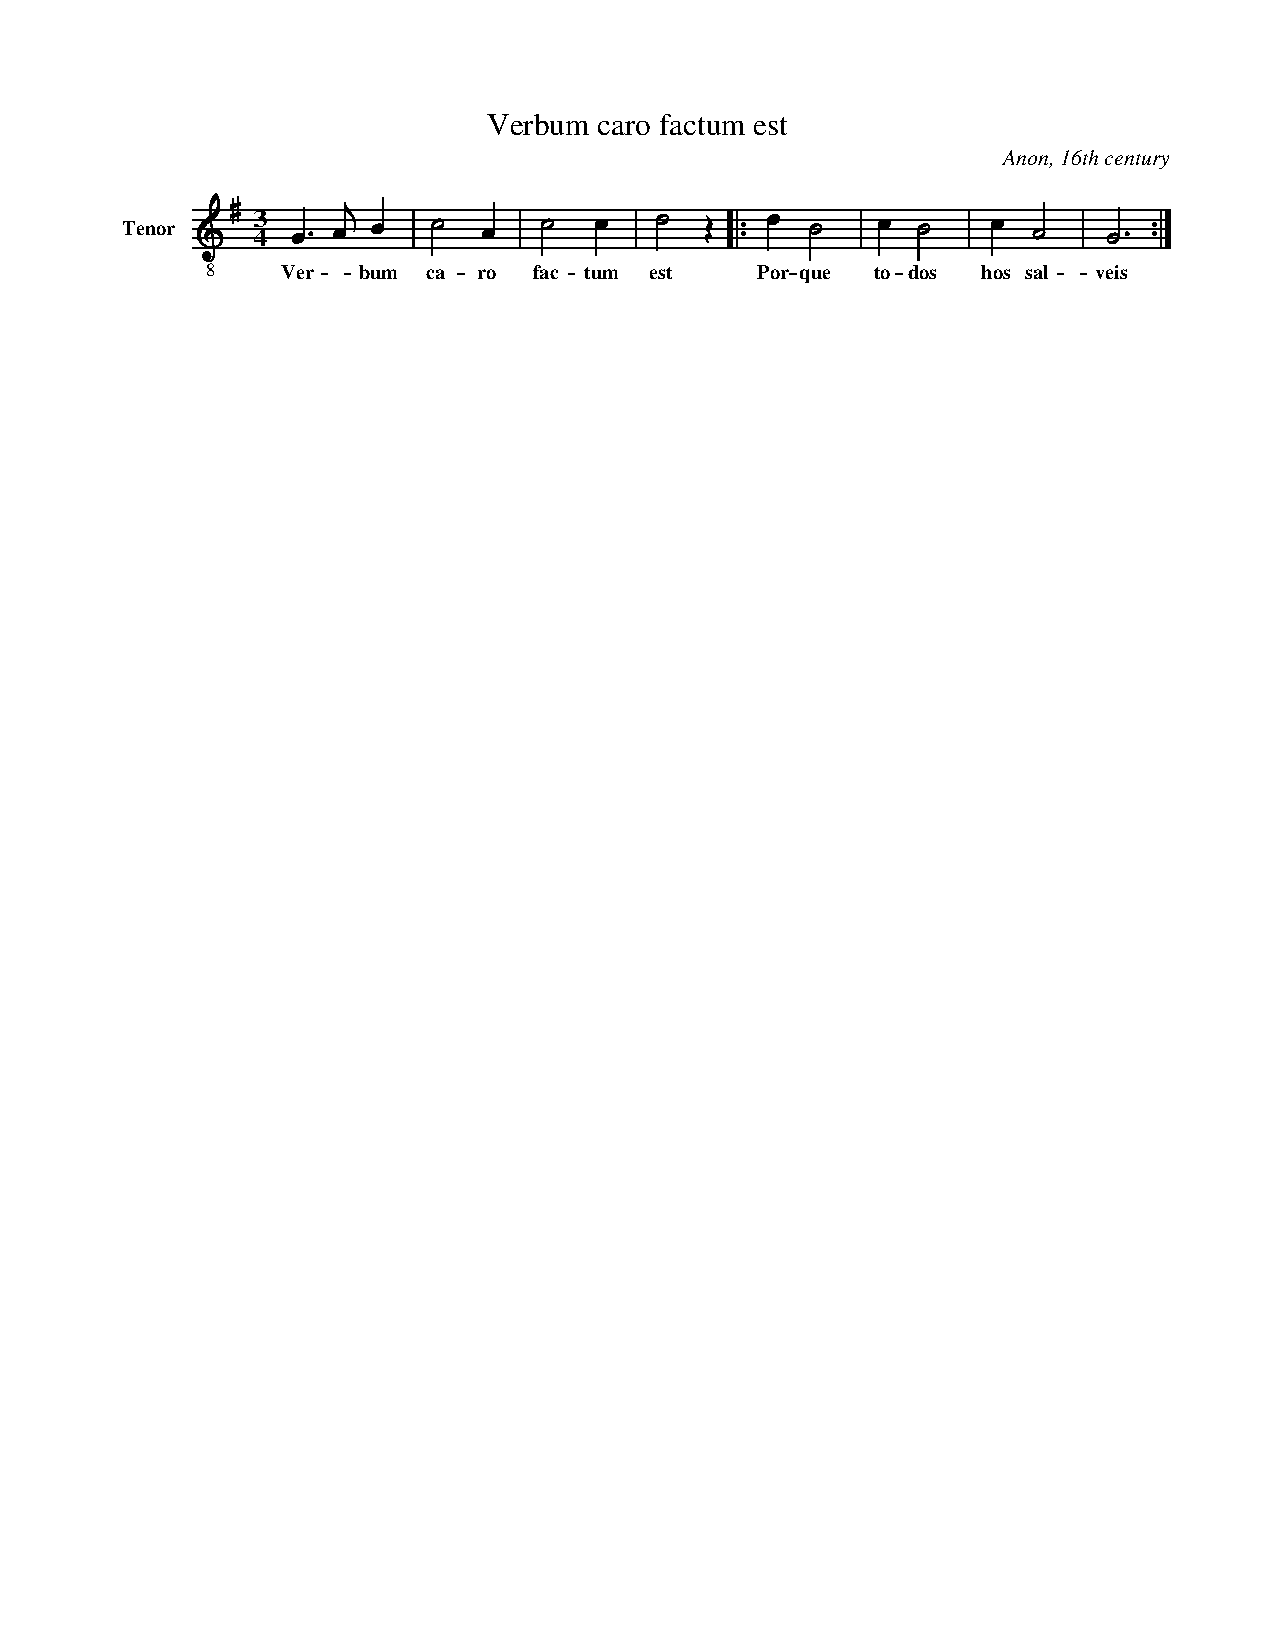
\includegraphics[width=0.8\textwidth, clip=true, trim = 15mm 231mm 17mm 0mm]{img/103.pdf}
    \caption{Verbum caro factum est: Section 1; Part 3 - Tenor (Score)}
  \end{center}
\end{figure}

\lstinputlisting[caption={Verbum caro factum est: Section 1; Part 1 \& 3},label={lst:verbum_s1_p1_p3_pasted},captionpos=t,abovecaptionskip=-\medskipamount]{misc/verbum_s1_p1_p3_pasted.tex}

\vspace{-1.30cm}
\begin{figure}[h]
  \begin{center}
    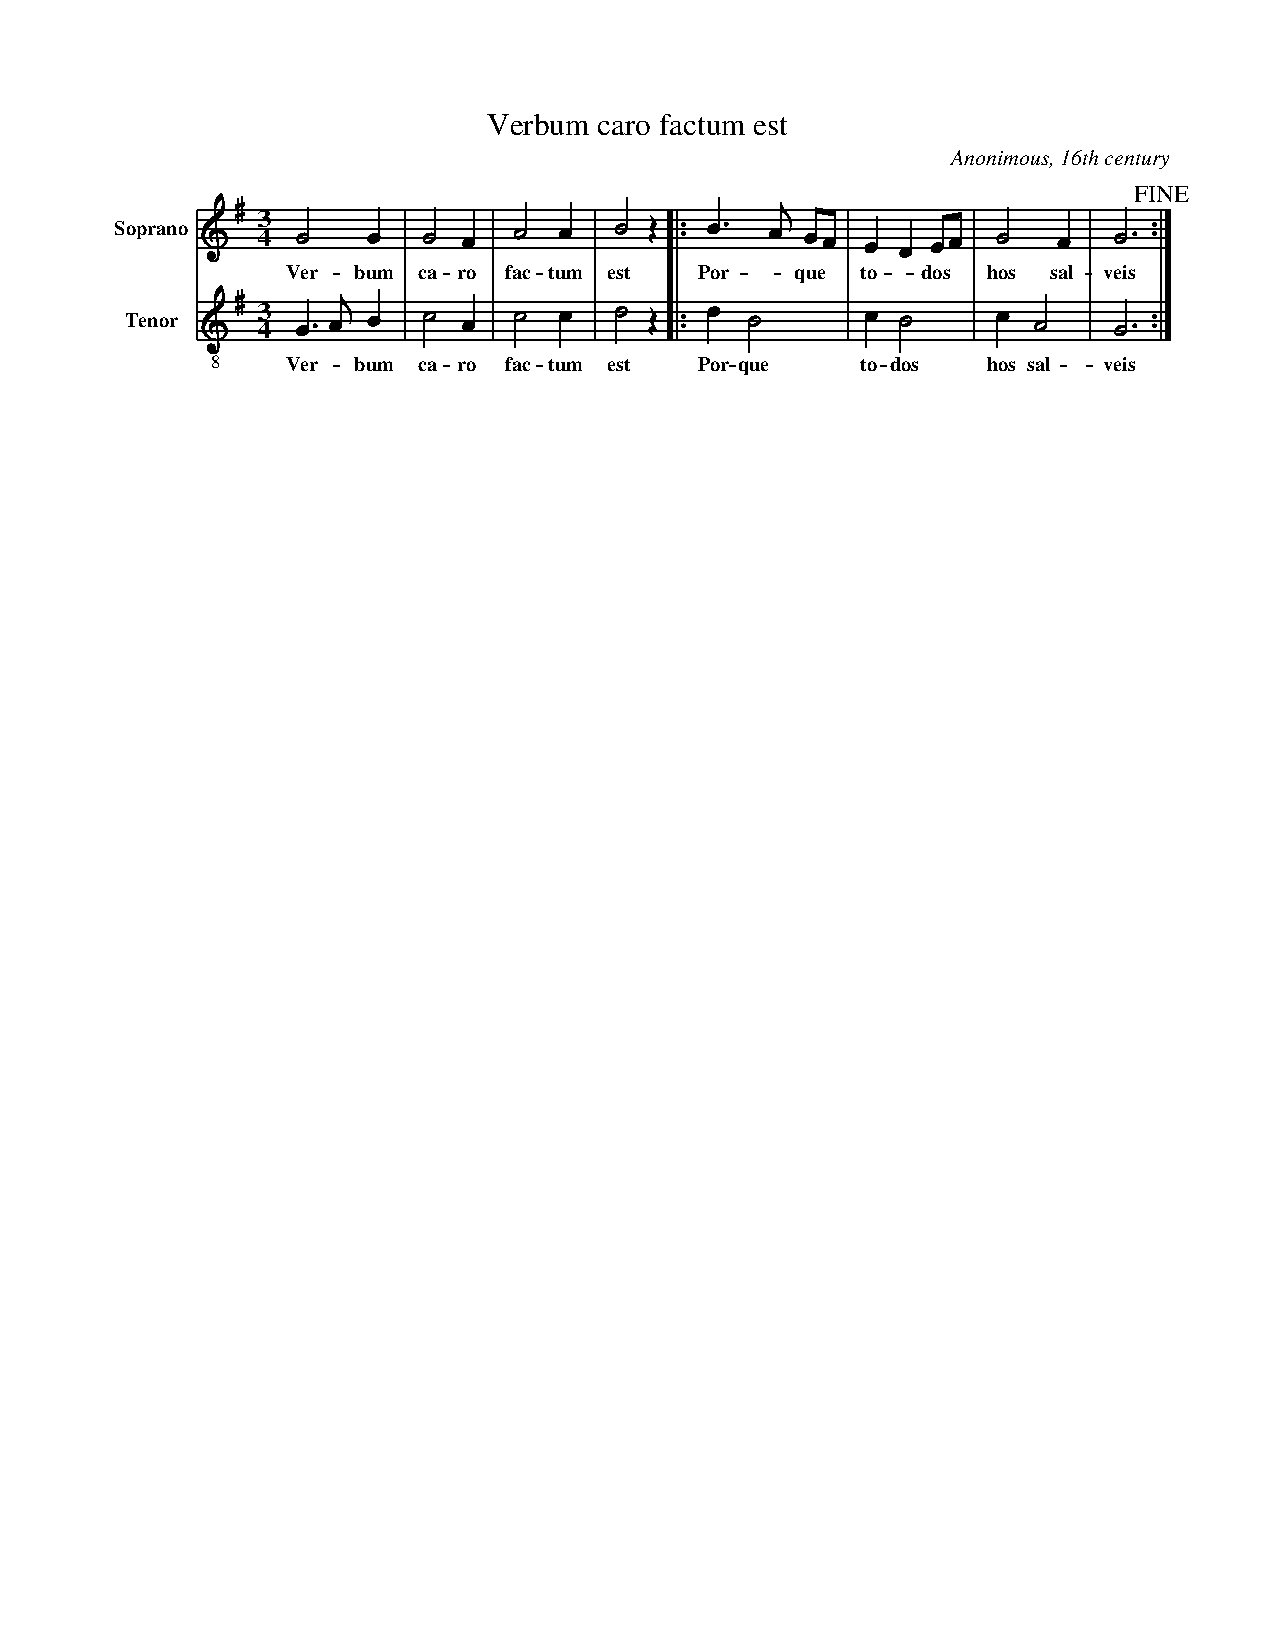
\includegraphics[width=0.8\textwidth, clip=true, trim = 15mm 210mm 15mm 0mm]{img/verbum_s1_p1_p3.pdf}
    \caption{Verbum caro factum est: Section 1; Part 1 \& 3 (Score)}
    \label{fig:verbum_s1_p1_p3_score}
  \end{center}
\end{figure}


\section{Cat ABC}
This tool is based on \unix{}'s \emph{cat}, as it consists in the concatenation of each tune one
after the other in the time perspective. In other words, any voice present in the second tune is
printed after the time offset corresponding to the end of the first tune, and so on.

Some design goals were established:

\begin{enumerate}
  \item The resulting tune's header derives from the first tune which has an actual tune written, in
  other words, at least one \emph{note}.
  \item The \context{} is updated every time a change is detected during the tune's traversal. It is
  a local data structure that comprises the \emph{current voice} and its \emph{key}, \emph{meter},
  \emph{length} and \emph{tempo}. The \emph{number of measures} per voice is recorded separately for
  each tune.
  \item Any \context{} change detected, like the \emph{key} or the \emph{meter}, is written to the
  resulting tune only if it is different from the current \context{}.
  \item For each tune, before appending it to the resulting tune, a verification for missing voices
  is made in the current tune and all prior to that. This way, \measurerests{} can be appended to any
  missing voice in order to ensure that the voice starts at the correct time offset.
  \item In the resulting tune, any voice that has fewer measures than the longest one is appended
  with the necessary \measurerests{} to match the longest.
\end{enumerate}

\subsection*{Algorithm}

\catabc{}'s algorithm is similar to \pasteabc{}'s except that after processing an \abc{} tune with
\dt{}, \measurerests{} may be appended to some voices before and after the actual tune is written.
Since all voices in an \abc{} file are written after the time offset corresponding to the end of the
previous \abc{} file, there may be music missing for some voices from one file to the other, thus
the need for \measurerests{} to fill those "holes".

So the algorithm has the following stages: \textbf{1)} retrieving the header for the resulting tune,
\textbf{2)} printing each tune and any necessary \measurerests{}. In the end, the output generated
is printed to the output.

An algorithmic description is made in algorithm \ref{alg:catabc}.

\begin{enumerate}
  \item The resulting tune's header comes from the first tune with at least one \emph{note} written.

  This stage does exactly the same as \pasteabc{}'s first stage.

  \item For each tune:

  \begin{enumerate}
    \item Applies \dt{} to the current tune;
    \item Appends \measurerests{} to every voice that is present in previous tunes and not in the current one;
    \item Appends \measurerests{} to every voice presented for the first time;
    \item Appends \dt{}'s output, which is the actual tune;
    \item Appends any necessary \measurerests{} to the processed tune (same as stage \textbf{3)} in
    \pasteabc{}'s main algorithm);
  \end{enumerate}

  \begin{program}
    When concatenating tune \emph{A} with tune \emph{B} and tune \emph{B} is being processed, step
    \textbf{b)} appends the \measurerests{} illustrated by the letter \emph{P1} and step \textbf{c)}
    appends the \measurerests{} illustrated by the letter \emph{P2}.

    % \vspace{-1.30cm}
    \begin{center}
      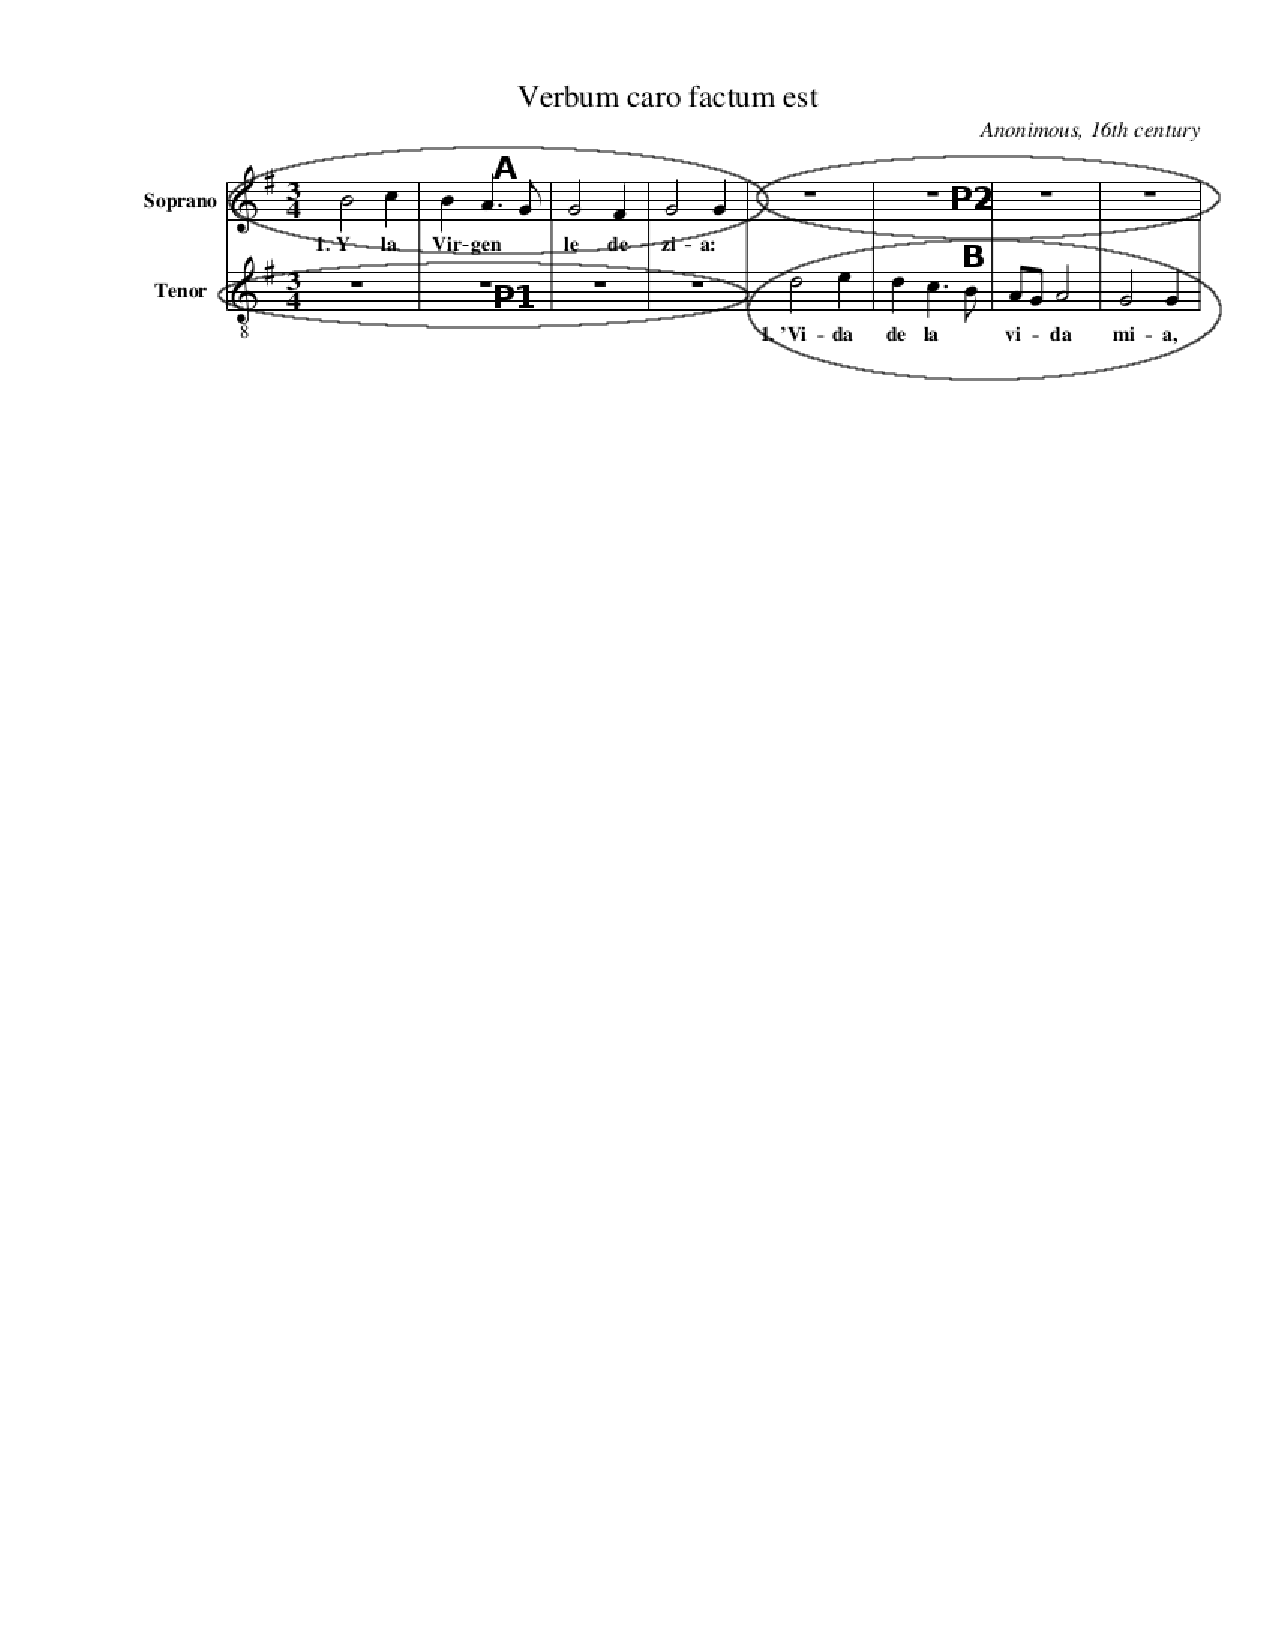
\includegraphics[width=0.8\textwidth, clip=true, trim = 15mm 213mm 0mm 10mm]{img/verbum_measures.pdf}
    \end{center}

    \caption{Appending necessary \measurerests{}}
  \end{program}

  Each individual result is concatenated into the resulting tune.\\

  The set of \abcdtrules{} used in this stage is the same as in \pasteabc{}'s second stage. However,
  \catabc{} provides two more options for concatenating tunes: inserting a number of \measurerests{}
  at the beginning of each tune (option \emph{-d}) and repeating each tune a number of times (option
  \emph{-r}).

  To implement the first option, some modifications were made to the set of \abcdtrules{}:

  \begin{itemize}
    \item The default transformation for each \abcelement{} is not \toabc{}, but instead a local
    function that, once for each voice, inserts a \measurerest{} with the request length before the
    element itself and also updates the \context{}'s measure count for that voice.
    \item The \context{}'s measure count update is made when a \emph{bar} or a \emph{mrest} is
    found.
  \end{itemize}

  Those modifications are described in table \ref{tab:cat_snd_stg_rules}.

  \begin{center}
    \begin{table}[h]
      \begin{tabular}{|p{2.5cm}|p{4.75cm}|p{8cm}|}
        \hline
        Actuator & Transformation (Perl) & Notes\\
        \hline
        \hline
        \emph{bar} & update\_measure\_count(1); insert\_canon\_delta(); &
        \emph{update\_measure\_count} is a local function that increments, in this case by 1, the
        \context{}'s measure count for the current voice. \emph{insert\_canon\_delta} is a local
        function that inserts a \measurerest{} before the element itself, once for each voice.
        \\
        \hline

        \hline
        \emph{mrest} & update\_measure\_count( \$sym->\{info\}->\{len\} - 1 );
        insert\_canon\_delta(); &
        \emph{\$sym} is the \abcelement{} currently being processed, a \measurerest{}.
        \emph{\$sym->\{info\}->\{len\}} is the number of measures in rest.
        \\
        \hline

        \hline
        \emph{-default} & insert\_canon\_delta(); &
        \\
        \hline
      \end{tabular}
      \caption{\abcdtrules{} for \catabc{}'s second stage}
      \label{tab:cat_snd_stg_rules}
    \end{table}
  \end{center}

  The second option is obtained by simply repeating steps \textbf{a} to \textbf{e} a requested
  number of times.
\end{enumerate}

\begin{algorithm}[h]
  \KwIn{abc\_tunes}
  \ForAll{$ tune \in abc\_tunes $}{
    $header \gets dt(tune,$ rules from table \ref{tab:paste_fst_stg_rules}$)$ \hfill //1)\\
  }
  \ForAll{$ tune \in abc\_tunes $}{
    \For{$ 0 .. $ value of \emph{-r} option }{
      $c\_tune \gets dt(tune,$ rules from tables \ref{tab:paste_snd_stg_rules} and \ref{tab:cat_snd_stg_rules}$)$ \hfill //2-a)\\
      $res \gets res$ ++ $add\_measures\_to\_missing\_voices()$ \hfill //2-b)\\
      $res \gets res$ ++ $add\_measures\_to\_new\_voices()$ \hfill //2-c)\\
      $res \gets res$ ++ $c\_tune$ \hfill //2-d)\\
      $res \gets res$ ++ $add\_measures()$ \hfill //2-e)\\
    }
  }
  \Return{$header$ ++ $res$}
  \caption{\catabc{}'s algorithm}
  \label{alg:catabc}
\end{algorithm}

\subsection*{Usage}

Listing \ref{lst:catabcman} shows \catabc{}'s manual.\\

\lstinputlisting[caption={\catabc{}'s manual},label={lst:catabcman},captionpos=t,abovecaptionskip=-\medskipamount]{misc/cat_manual.tex}

Listing \ref{lst:cat_abc_by_example} shows a usage example for \catabc{}. It reads tunes
\textbf{201.abc} (listing \ref{lst:verbum_s2_p1}) and \textbf{303.abc} (listing
\ref{lst:verbum_s3_p3}) and the output is shown in listing \ref{lst:verbum_s2_p1_s3_p3_cated} with
its respective score (figure \ref{fig:verbum_s2_p1_s3_p3}).\\

\begin{lstlisting}[caption={\catabc{} by example},label={lst:cat_abc_by_example},captionpos=t,abovecaptionskip=-\medskipamount]
cat_abc 201.abc 303.abc
\end{lstlisting}

\lstinputlisting[caption={Verbum caro factum est: Section 2; Part 1 - Soprano},label={lst:verbum_s2_p1},captionpos=t,abovecaptionskip=-\medskipamount]{misc/201.tex}

\vspace{-1.30cm}
\begin{figure}[h]
  \begin{center}
    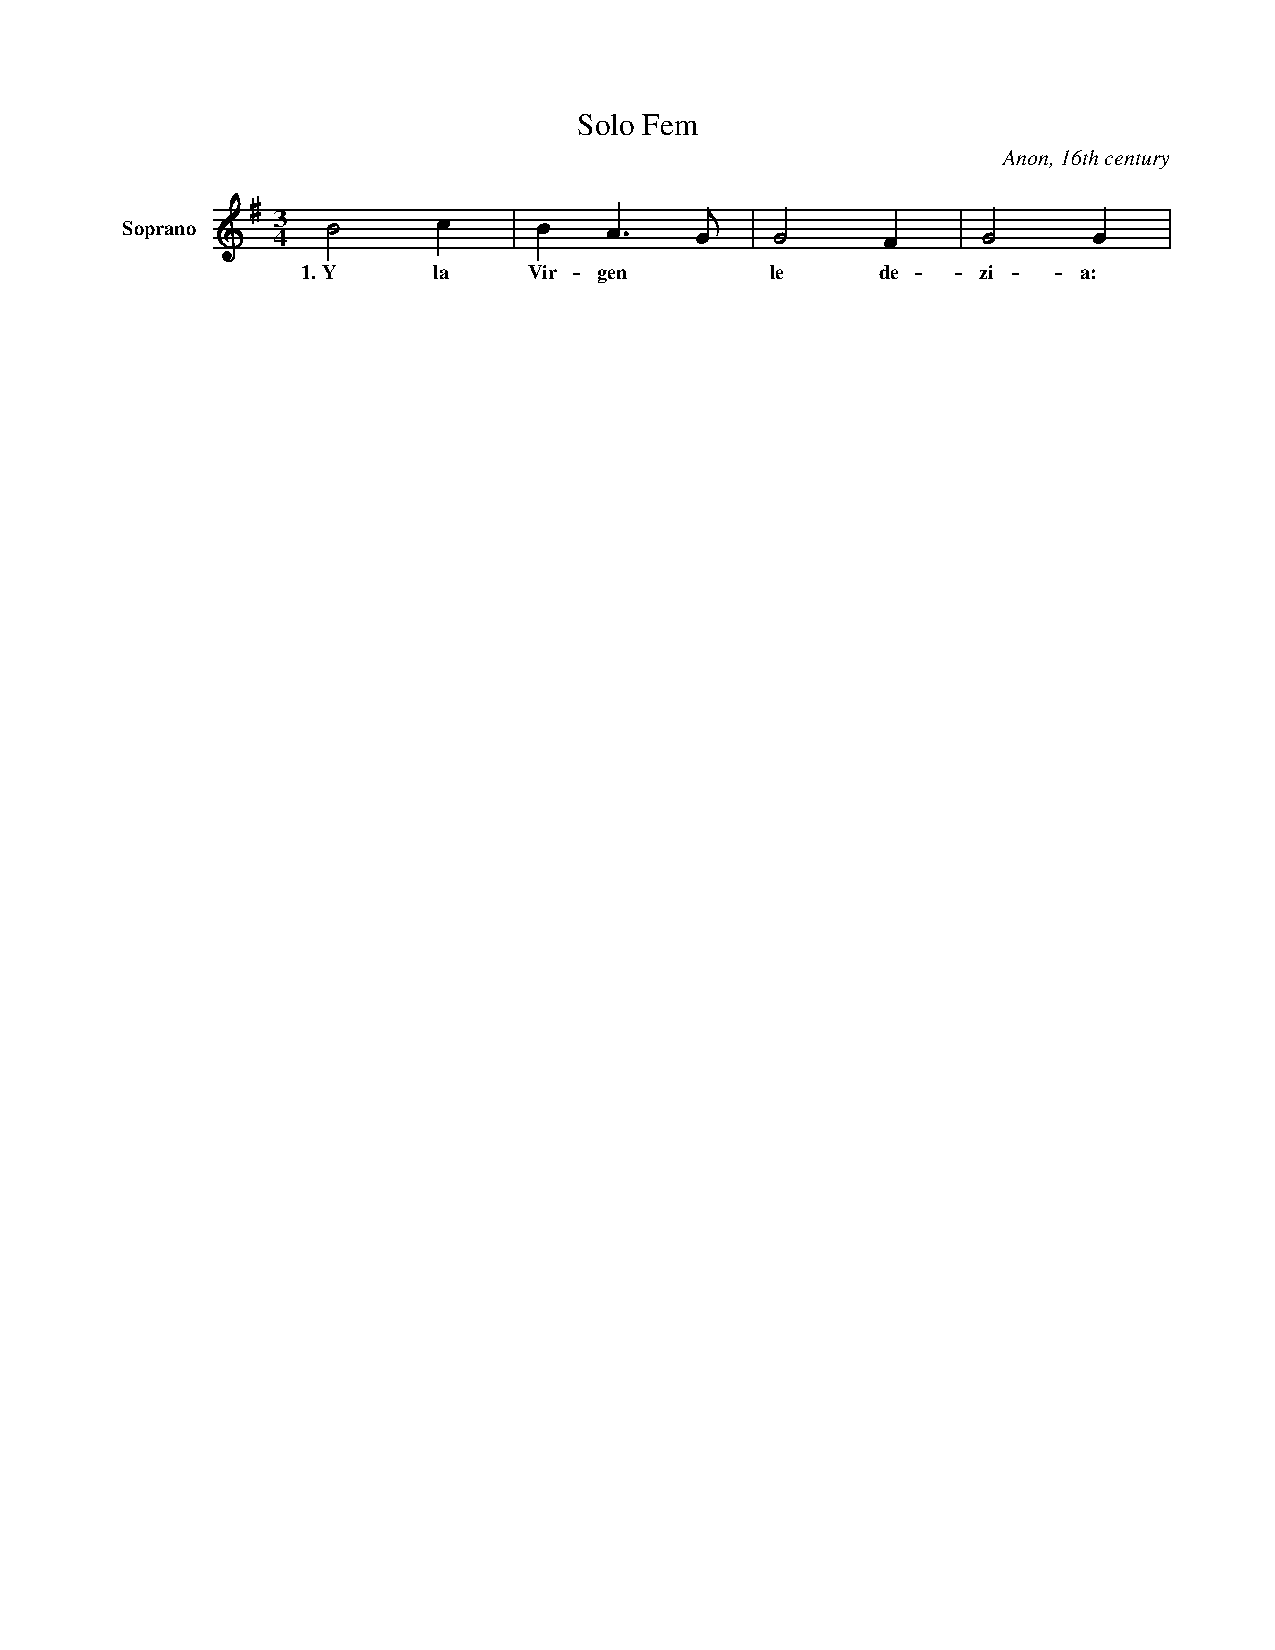
\includegraphics[width=0.8\textwidth, clip=true, trim = 15mm 231mm 0mm 0mm]{img/201.pdf}
    \caption{Verbum caro factum est: Section 2; Part 1 - Soprano (Score)}
  \end{center}
\end{figure}

\lstinputlisting[caption={Verbum caro factum est: Section 3; Part 3 - Tenor},label={lst:verbum_s3_p3},captionpos=t,abovecaptionskip=-\medskipamount]{misc/303.tex}

% \vspace{-1.30cm}
\begin{figure}[H]
  \begin{center}
    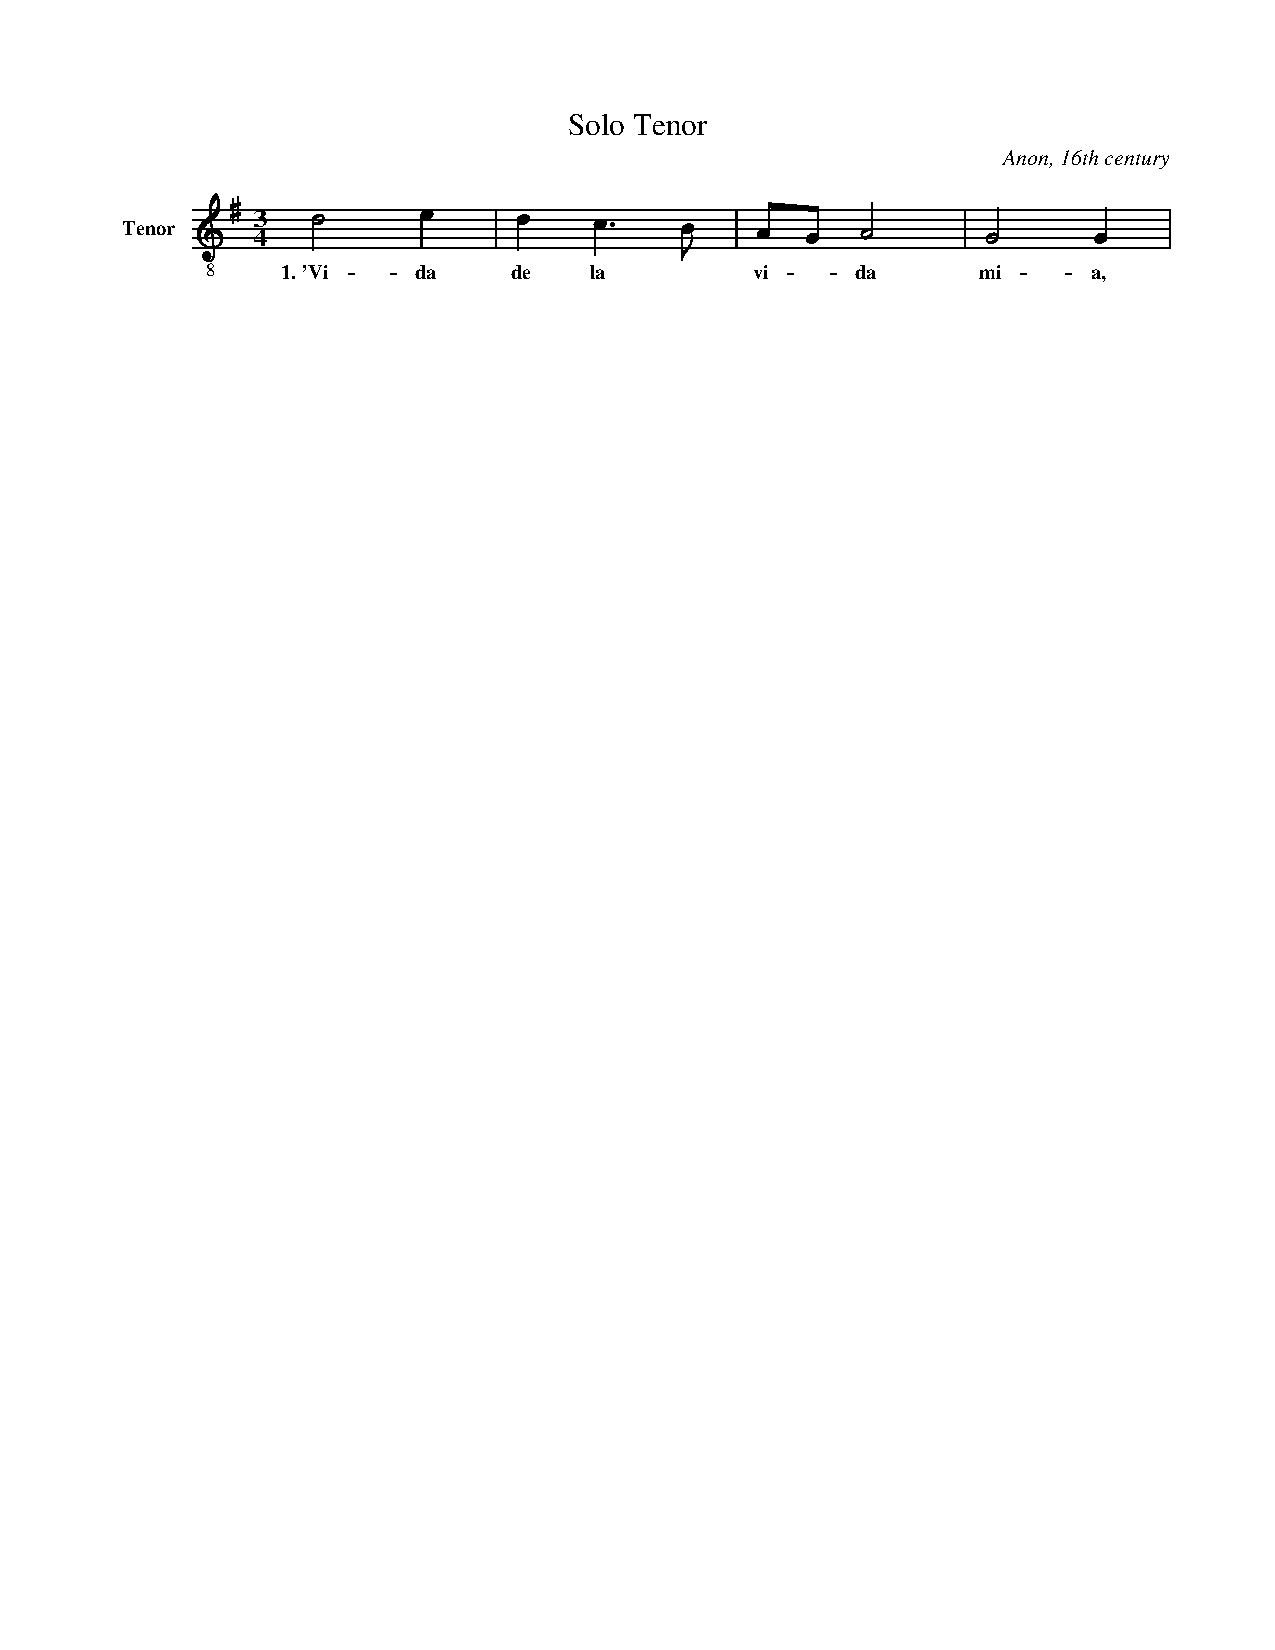
\includegraphics[width=0.8\textwidth, clip=true, trim = 15mm 231mm 0mm 0mm]{img/303.pdf}
    \caption{Verbum caro factum est: Section 3; Part 3 - Tenor (Score)}
  \end{center}
\end{figure}

\lstinputlisting[caption={Verbum caro factum est: Section 2; Part 1 \& Section 3: Part 3},label={lst:verbum_s2_p1_s3_p3_cated},captionpos=t,abovecaptionskip=-\medskipamount]{misc/verbum_s2_p1_s3_p3_cated.tex}

\vspace{-1.50cm}
\begin{figure}[H]
  \begin{center}
    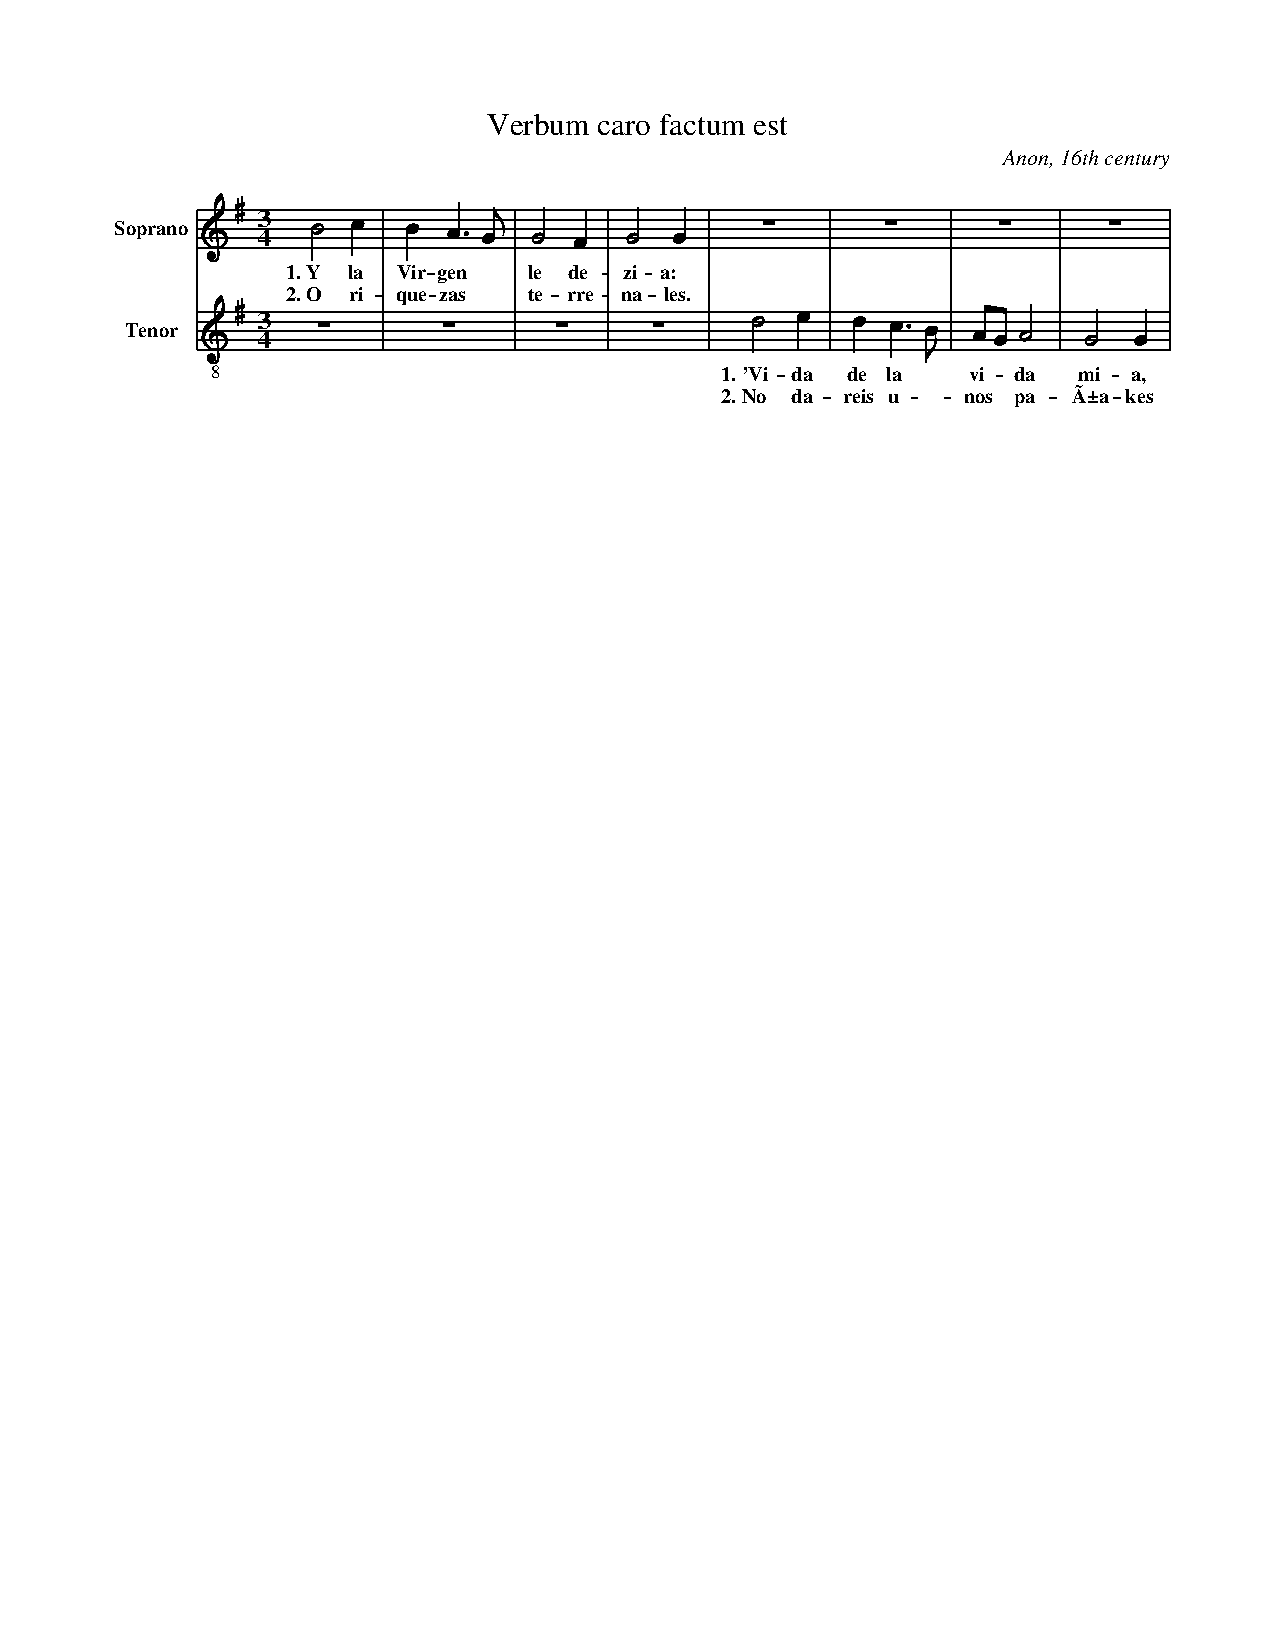
\includegraphics[width=0.8\textwidth, clip=true, trim = 18mm 210mm 16mm 0mm]{img/verbum_s2_p1_s3_p3.pdf}
    \caption{Verbum caro factum est: Section 2; Part 1 \& Section 3: Part 3 (Score)}
    \label{fig:verbum_s2_p1_s3_p3}
  \end{center}
\end{figure}


\section{Learning ABC}
When there is a multi-voice score, like a four part choir, it is important to, for instance, the
Soprano to be able to study her part individually. Sometimes there's the need to hear all the other
parts except hers, so that she may know what the rest is going to sound. Other times the opposite is
what is needed.

The \learningabc{} tool generates two \abc{} scores whose goal is to help musicians in individual
rehearsal of multi-voice music for studying purposes. One reduces the volume of a particular voice
and the other increases the volume of a particular voice and reduces the volume of the remaining
voices.

\subsection*{Algorithm}

\learningabc{}'s algorithm consists of 3 stages that are applied to each tune.

An algorithmic description is made in algorithm \ref{alg:learningabc}.\\

For each tune:
\begin{enumerate}
  \item \textbf{Retrieve voice data}

  In this stage, the tune is processed by \dt{}, in which each voice's name, channel and program
  (instrument) are stored to be used in the following stages.

  The set of \abcdtrules{} is shown in table \ref{tab:learning_abc_fst_stage}.

  \begin{center}
    \begin{table}[h]
      \begin{tabular}{|p{3cm}|p{5cm}|p{7.5cm}|}
        \hline
        Actuator & Transformation (Perl) & Notes\\
        \hline
        \hline
        \emph{V:} & store\_channel\_and\_name(); & Local function that stores each voice's channel
        and name.
        \\
        \hline

        \hline
        \emph{MIDI::program} & store\_program(); & Local function that stores each voice's program.
        \\
        \hline
      \end{tabular}
      \caption{\abcdtrules{} for \learningabc{}'s first stage}
      \label{tab:learning_abc_fst_stage}
    \end{table}
  \end{center}

  \item \textbf{All but one}

  In \abc{}, it is possible to add commands to control audio properties through the use of \midi{}
  directives (\emph{\%\%MIDI}, followed by different parameters) that \abctomidi{} recognizes.

  In this stage, the tune is processed by \dt{}, in which a \midi{} directive to reduce the volume
  of the voice is inserted. To be more precise, a change-volume \midi{} directive (\emph{\%\%MIDI
  control 7 NewVolume}, where \emph{NewVolume} is a number between (0-127)- is appended after the
  voice definition.

  In the end, the processed tune is written to a new \abc{} file.

  The set of \abcdtrules{} is shown in table \ref{tab:learning_abc_snd_stage}.

  \begin{center}
    \begin{table}[h]
      \begin{tabular}{|p{2.25cm}|p{6.75cm}|p{6.5cm}|}
        \hline
        Actuator & Transformation (Perl) & Notes\\
        \hline
        \hline
        \emph{V:\$req\_voice} & toabc() . "\%\%MIDI control 7 \$min\_volume\textbackslash{}n"); &
        \emph{\$req\_voice} keeps the voice requested when calling \learningabc{}.
        \\
        \hline
      \end{tabular}
      \caption{\abcdtrules{} for \learningabc{}'s second stage}
      \label{tab:learning_abc_snd_stage}
    \end{table}
  \end{center}

  \item \textbf{Just one}

  In this stage, the tune is processed by \dt{}, in which, for each voice, three \midi{} directives
  are inserted after the \emph{X:} statement. The first is a select-channel directive
  (\emph{\%\%MIDI channel Channel}, where \emph{Channel} is a number between (1-16)), the second a
  select-program directive (\emph{\%\%MIDI program Channel Program}, where \emph{Program} is the
  instrument (0-127) for channel \emph{Channel}) and the third is a change-volume directive to
  reduce or increase the voice's volume. Furthermore, the select-channel directive is also appended
  to the voice statement so that \abctomidi{} can make the association between the voice and the
  channel when reproducing.

  In the end, the processed tune is written to a new \abc{} file.

  The set of \abcdtrules{} is shown in table \ref{tab:learning_abc_trd_stage}.

  \begin{center}
    \begin{table}[h]
      \begin{tabular}{|p{1.5cm}|p{7.5cm}|p{6.5cm}|}
        \hline
        Actuator & Transformation (Perl) & Notes\\
        \hline
        \hline
        \emph{X:} & set\_volume(); & Local function that sets the volume by appending the three
        \midi{} directives mentioned before for each voice.
        \\
        \hline

        \hline
        \emph{V:} & toabc() . "\%\%MIDI channel
        \$voice\_channel\{\$c\_voice\}\{channel\}\textbackslash{}n"; & Appends the select-channel
        directive after its corresponding voice.
        \\
        \hline
      \end{tabular}
      \caption{\abcdtrules{} for \learningabc{}'s third stage}
      \label{tab:learning_abc_trd_stage}
    \end{table}
  \end{center}
\end{enumerate}

\begin{algorithm}[h]
  \KwIn{abc\_tunes}
  \ForAll{$ tune \in abc\_tunes $}{
    $dt(tune,$ rules from table \ref{tab:learning_abc_fst_stage}$)$ \hfill //1)\\
    $just\_one \gets dt(tune,$ rules from table \ref{tab:learning_abc_snd_stage}$)$ \hfill //2)\\
    $write\_to\_file(just\_one)$ \hfill //2)\\
    $all\_but\_one \gets dt(tune,$ rules from table \ref{tab:learning_abc_trd_stage}$)$ \hfill //3)\\
    $write\_to\_file(all\_but\_one)$ \hfill //3)\\
  }
  \Return{}
  \caption{\learningabc{}'s algorithm}
  \label{alg:learningabc}
\end{algorithm}

\subsection*{Usage}

Listing \ref{lst:learningabcman} shows \learningabc{}'s manual.\\

\lstinputlisting[caption={\learningabc{}'s manual},label={lst:learningabcman},captionpos=t,abovecaptionskip=-\medskipamount]{misc/learning_manual.tex}

Listing \ref{lst:learningabcbyexample} shows a usage example for \learningabc{}. It reads tune
\textbf{100.abc} (listing \ref{lst:verbum_s1}) and the output is shown in listing
\ref{lst:100_all_but_tenor} and \ref{lst:100_just_tenor}.\\

\begin{lstlisting}[caption={\learningabc{} by example},label={lst:learningabcbyexample},captionpos=t,abovecaptionskip=-\medskipamount]
learning_abc -v=Tenor -min=25 100.abc
\end{lstlisting}

\begin{center}
  \begin{minipage}{.49\textwidth}
    \lstinputlisting[caption={100.abc},label={lst:verbum_s1},captionpos=t,abovecaptionskip=-\medskipamount]{misc/verbum_s1.tex}
  \end{minipage}
  \hfill
  \begin{minipage}{.49\textwidth}
    \lstinputlisting[caption={100\_all\_but\_Tenor.abc},label={lst:100_all_but_tenor},captionpos=t,abovecaptionskip=-\medskipamount]{misc/100_all_but_Tenor.tex}
  \end{minipage}
\end{center}

Note the \midi{} command \texttt{\%\%MIDI control 7 25} after \texttt{V:3} in listing
\ref{lst:100_all_but_tenor}. That way, voice "Tenor" is going to be attenuated when \abctomidi{}
reproduces the score.\\

\lstinputlisting[caption={100\_just\_Tenor.abc},label={lst:100_just_tenor},captionpos=t,abovecaptionskip=-\medskipamount]{misc/100_just_Tenor.tex}


\section{Wc ABC}
This tool, is similar to \unix{}'s wc, in the sense that it prints voices, measures and
notes/pitches per voice counts for each \abc{} file.

This tool generates a textual summary of the counts made.
For each tune it prints:
\begin{itemize}
  \item number of voices
  \item for each voice:
  \begin{itemize}
    \item total number of notes
    \item total number of measures
    \item number of occurrences of a certain note (pitch)
  \end{itemize}
\end{itemize}

\subsection*{Algorithm}

\wcabc{}'s algorithm consists in processing each tune with \dt{} in order to produce the desired
counts. In the end an output is generated with the produced data.

An algorithmic description is made in algorithm \ref{alg:wcabc}.

The voice count is updated when the \emph{voice} element is found, the note and pitch counts are
updated when the \emph{note} element is found and the measure count is updated when the \emph{bar}
element is found. The set of \abcdtrules{} is shown in table \ref{tab:wc_abc_rules}.

\begin{center}
  \begin{table}[h]
    \begin{tabular}{|p{2cm}|p{5cm}|p{7.5cm}|}
      \hline
      Actuator & Transformation (Perl) & Notes\\
      \hline
      \hline
      \emph{V:} & update\_voice\_count(); & Local function that increments the voice count when a
      new voice is found.
      \\ \cline{1-2}
      \hline

      \hline
      \emph{note} & update\_note\_count(); & Local function that increments the note and pitch
      count. For the pitch name, it uses \abcdt{}'s function \emph{get\_pitch\_name()}.
      \\ \cline{1-2}
      \hline

      \hline
      \emph{bar} & update\_measure\_count(); & Local function that increments the measure count
      according to the bar number.
      \\ \cline{1-2}
      \hline
    \end{tabular}
    \caption{\abcdtrules{} for \wcabc{}}
    \label{tab:wc_abc_rules}
  \end{table}
\end{center}

\begin{algorithm}[h]
  \KwIn{abc\_tunes}
  \ForAll{$ tune \in abc\_tunes $}{
    $dt(tune,$ rules from table \ref{tab:wc_abc_rules}$)$\\
  }
  $res \gets create\_output()$\\
  \Return{$res$}
  \caption{\wcabc{}'s algorithm}
  \label{alg:wcabc}
\end{algorithm}

\subsection*{Usage}

Listing \ref{lst:wcabcman} shows \wcabc{}'s manual.\\

\lstinputlisting[caption={\wcabc{}'s manual},label={lst:wcabcman},captionpos=t,abovecaptionskip=-\medskipamount]{misc/wc_manual.tex}

Listing \ref{lst:wcabcbyexample} shows a usage example for \wcabc{}. It reads the tune generated by
\pasteabc{} (listing \ref{lst:verbum_s1_p1_p3_pasted}) and the output is shown in listing
\ref{lst:wc_output}.\\

\begin{lstlisting}[caption={\wcabc{} by example},label={lst:wcabcbyexample},captionpos=t,abovecaptionskip=-\medskipamount]
wc_abc 101_103.abc
\end{lstlisting}

\lstinputlisting[caption={\wcabc{}'s output},label={lst:wc_output},captionpos=t,abovecaptionskip=-\medskipamount]{misc/verbum_s1_p1_p3_pasted_wc.tex}

\wcabc{} reports that there are 2 voices. Voice with \emph{id} 1 has 8 measures, a total of 18 notes
and 6 \emph{G}'s, 4 \emph{F}'s, 3 \emph{A}'s, 3 \emph{E}'s, 2 \emph{B}'s and 1 \emph{D}.  The
interpretation for voice with \emph{id} 3 is analogous.


\section{Detect Errors ABC}
\abc{} is a textual music notation, therefore it is very common for an \abc{} score to have
syntactical errors, such as, having more beats in a measure than it can hold.

There are three kinds of behavior when facing an error: correct it immediately (e.g.: insert a bar
when it's missing); warn the user of the error's existence; and comment the error and annotate a
\emph{FIXME} comment so that the user can locate and fix the error manually.

Due to time limitations, only one behavior is adopted in \detecterrorsabc{}, which is to warn the
user. So, for each file, it detects errors and produces an output with error messages along with the
voice and measure number where they occurred.

\detecterrorsabc{} will expose the following errors:

\begin{description}
  \item[Incomplete/Overflowing measure] \hfill \\
    A measure is a segment of time defined by a given number of beats which is delimited by a
    \emph{bar} element. The number of beats in a measure is determined by the \emph{Meter (M:)}
    previously defined.

    The first metrically complete measure within a score is the first measure. When the score begins
    with an anacrusis (an incomplete measure at the head of a score), the first measure is the
    following measure.

    So, the number of beats (the length of all notes and rests) in a measure (except if it is an
    anacrusis) must be equal to that measure's defined length.

  \item[Last \abc{} element per voice isn't a bar] \hfill \\
    \abc{} allows a score to not having a \emph{bar} at the end of a voice, however, it isn't
    considered a good practice in modern music notation.

    Therefore, a voice must finish with a \emph{bar} element, in other words, the last
    \abcelement{}, except \emph{eoln}, for a voice has to be a \emph{bar}.

  \item[Different number of measures per voice] \hfill \\
    All voices must have the same number of measures.

  \item[Different key definitions per measure] \hfill \\
    In modern music, there are certain properties that apply to many elements simultaneously, for
    instance, in a multi-voice score, the second measure is the second measure for all voices, as
    well as the key, among others. However, in \abc{}, that assumption may be ignored.

    Thus, for each measure, the key must be the same for all voices.

\end{description}

\subsection*{Algorithm}

\detecterrorsabc{}'s algorithm consists of 2 stages that are applied to each tune.

An algorithmic description is made in algorithm \ref{alg:detecterrorsabc}.\\

For each tune:

\begin{enumerate}
  \item \textbf{Retrieve data and detect incomplete/overflowing measures}

  In this stage, the tune is processed by \dt{}, in which each voice's \emph{last \abc {} element},
  \emph{number of measures} and the \emph{key per measure} are stored to be used in the following
  stage.

  It also stores the \emph{current measure's real length} in order to detect incomplete/overflowing
  measures. In order to accomplish the latter, when the \emph{bar} element is found, it compares the
  \emph{current measure's real length} with the current measure's defined length.

  The set of \abcdtrules{} is shown in table \ref{tab:detect_errors_abc_fst_stage}.

  \begin{center}
    \begin{table}[h]
      \begin{tabular}{|p{2cm}|p{6cm}|p{7.5cm}|}
        \hline
        Actuator & Transformation (Perl) & Notes\\
        \hline
        \hline
        \emph{in\_tune} & update\_data(\{\}); & Local function that sets the current element as the
        current voice's last \abc{} element.
        \\
        \hline

        \hline
        \emph{note} & update\_data(\{meas\_dur => 1, n\_meas => 1\}); & Local function that sets the
        current element as the current voice's last \abc{} element. When \emph{meas\_dur} is 1, it
        increments the current measure's real length with the element's value. When \emph{n\_meas}
        is 1, it updates the current voice's number of measures.
        \\
        \hline

        \hline
        \emph{rest} & update\_data(\{meas\_dur => 1, n\_meas => 1\}); &
        \\
        \hline

        \hline
        \emph{mrest} & update\_data(\{key => 1\}); & Local function that sets the current element as
        the current voice's last \abc{} element. When \emph{key} is 1, it updates the key for all
        measures that \emph{mrest} covers.
        \\
        \hline

        \hline
        \emph{bar} & \$ret .= check\_measure\_length(); update\_data(\{n\_meas => 1, key => 1\}); &
        \emph{check\_measure\_length} is a local function that detects if the current measure is
        incomplete or overflowing and returns an error message in case it finds one.
        \\
        \hline

        \hline
        \emph{eoln} & q\{\}; & The end of a line won't be set as a voice's last element.
        \\
        \hline
      \end{tabular}
      \caption{\abcdtrules{} for \detecterrorsabc{}'s first stage}
      \label{tab:detect_errors_abc_fst_stage}
    \end{table}
  \end{center}

  \item \textbf{Detect the remaining syntactical errors}

  It detects if the tune's last \abc{} element for all voices is a \emph{bar} and if the number of
  measures is the same for all voices. Error messages are produced in case errors are found.

  If no errors were found until this moment, then the detection for different key definitions per
  measure proceeds.
\end{enumerate}

\begin{algorithm}[H]
  \KwIn{abc\_tunes}
  \ForAll{$ tune \in abc\_tunes $}{
    $dt(tune,$ rules from table \ref{tab:detect_errors_abc_fst_stage}$)$ \hfill //1)\\
    $res \gets res$ ++ $detect\_remaining\_errors()$ \hfill //2)\\
  }
  \Return{$res$}
  \caption{\detecterrorsabc{}'s algorithm}
  \label{alg:detecterrorsabc}
\end{algorithm}

\subsection*{Usage}

Listing \ref{lst:detecterrorsabcman} shows \detecterrorsabc{}'s manual.\\

\lstinputlisting[caption={\detecterrorsabc{}'s manual},label={lst:detecterrorsabcman},captionpos=t,abovecaptionskip=-\medskipamount]{misc/detect_errors_manual.tex}

Listing \ref{lst:detecterrorsabcbyexample} shows a usage example for \detecterrorsabc{}. It reads
the tune \textbf{100\_errors.abc} (listing \ref{lst:100errors}) and the output is shown in listing
\ref{lst:detect_errors_output}.\\

\begin{lstlisting}[caption={\detecterrorsabc{} by example},label={lst:detecterrorsabcbyexample},captionpos=t,abovecaptionskip=-\medskipamount]
detect_errorsabc 100_errors.abc
\end{lstlisting}

\lstinputlisting[caption={100.abc with errors},label={lst:100errors},captionpos=t,abovecaptionskip=-\medskipamount]{misc/100_errors.tex}

\lstinputlisting[caption={\detecterrorsabc{}'s output},label={lst:detect_errors_output},captionpos=t,abovecaptionskip=-\medskipamount]{misc/detect_errors_output.tex}


\section{Find Chords ABC}
\findchordsabc{} searches voices for melodically expressed chord formations (chords formed from a
list of consecutive notes) such as a \emph{dominant seventh} or a \emph{major triad}. It then
inserts an accompaniment chord with the labeled chord in the first note of a found chord.

\subsection*{Algorithm}

\findchordsabc{}'s algorithm consists in processing each tune with \dt{} in order to find the
request chord formations. In the end, it returns the original tune with a labeled chord inserted as
accompaniment chord into the first note of all chords found.

An algorithmic description is made in algorithm \ref{alg:findchordsabc}.\\

The set of \abcdtrules{} has only one rule. Basically, for each visited \emph{note} element, all
consecutive notes in that measure are collected in order to form a chord and test if its formation
has been requested by the user. The actuator isn't static though, i.e. the user may limit the search
to a particular voice, consequently a \emph{voice restriction} needs to be added to the \emph{note}
actuator.

The set of \abcdtrules{} is shown in table \ref{tab:find_chords_abc_stage}.

\begin{center}
  \begin{table}[h]
    \begin{tabular}{|p{2cm}|p{7cm}|p{6cm}|}
      \hline
      Actuator & Transformation (Perl) & Notes\\
      \hline
      \hline
      \multirow{15}{*}{\$note\_act}
      & my @notes = find\_consecutive\_notes\_in\_measure( { skip\_unisons => 1, skip\_octaves => 1,
      skip\_rests   => 1, no\_undef     => 1 } );& \abcdt{}'s function that gets a list of
      consecutive notes, skipping unisons, octaves, and rests.
      \\

      & search\_requested\_chords(@notes); & Local function that searches for each requested chord
      formation by taking \emph{X} consecutive notes at a time from \emph{@notes} and creating the
      chord to be tested against the requested chord formations. \emph{X} is a number taken from a
      table that associates a chord formation to the number of notes that form it.
      \\

      & to\_abc(); & Prints the \emph{note} element that may have or not a labeled chord as
      accompaniment chord.
      \\
      \hline
    \end{tabular}
    \caption{\abcdtrules{} for \findchordsabc{}}
    \label{tab:find_chords_abc_stage}
  \end{table}
\end{center}

To test a chord's formation, some \abcdt{} functions are being used, namely, \emph{root()},
\emph{get\_pitch\_name()}, \emph{is\_major\_triad()}, \emph{is\_minor\_triad()},
\emph{is\_dominant\_seventh()}. These are explained in appendix \ref{sec:abcdt_functions}.

\findchordsabc{} also allows the user to specify which voices shouldn't be searched. That feature is
translated into a set of \abcdtrules{} for each of the specified voices, in which, each rule assigns
\toabc{} to a \emph{note} element with a \emph{voice restriction}. So, if \emph{\$ex\_voice} is a
particular voice to be excluded from the search, then the additional rule in table
\ref{tab:find_chords_abc_additional_rule} would be added to the existing set of \abcdtrules{}.

\begin{center}
  \begin{table}[h]
    \begin{tabular}{|p{4.5cm}|p{4cm}|p{6.5cm}|}
      \hline
      Actuator & Transformation (Perl) & Notes\\
      \hline
      \hline
      "V:\$ex\_voice" . '::note' & to\_abc(); & No chord formations will be searched in this
      particular voice.\\
      \hline
    \end{tabular}
    \caption{Additional \abcdtrules{} for \findchordsabc{}}
    \label{tab:find_chords_abc_additional_rule}
  \end{table}
\end{center}

\begin{algorithm}[H]
  \KwIn{abc\_tunes}
  \ForAll{$ tune \in abc\_tunes $}{
    $res \gets res$ ++ $dt(tune,$ rules from tables \ref{tab:find_chords_abc_stage} and \ref{tab:find_chords_abc_additional_rule} $)$\\
  }
  \Return{$res$}
  \caption{\findchordsabc{}'s algorithm}
  \label{alg:findchordsabc}
\end{algorithm}

\subsection*{Usage}

Listing \ref{lst:findchordsabcman} shows \findchordsabc{}'s manual.\\

\lstinputlisting[caption={\findchordsabc{}'s manual},label={lst:findchordsabcman},captionpos=t,abovecaptionskip=-\medskipamount]{misc/findchords_manual.tex}

Listing \ref{lst:findchords_abc_by_example} shows a usage example for \findchordsabc{}. It reads
tunes \textbf{100\_with\_maj\_t.abc} (listing \ref{lst:verbum_s1_with_maj_t}) and the output is
shown in listing \ref{lst:verbum_s1_with_chords}.\\

\begin{lstlisting}[caption={\findchordsabc{} by example},label={lst:findchords_abc_by_example},captionpos=t,abovecaptionskip=-\medskipamount]
find_chords_abc 100_with_maj_t.abc
\end{lstlisting}

\begin{center}
  \begin{minipage}{.49\textwidth}
    \lstinputlisting[caption={100\_with\_maj\_t.abc},label={lst:verbum_s1_with_maj_t},captionpos=t,abovecaptionskip=-\medskipamount]{misc/verbum_s1_with_maj_t.tex}
  \end{minipage}
  \hfill
  \begin{minipage}{.49\textwidth}
    \lstinputlisting[caption={\findchordsabc{}'s output},label={lst:verbum_s1_with_chords},captionpos=t,abovecaptionskip=-\medskipamount]{misc/verbum_s1_with_chords.tex}
  \end{minipage}
\end{center}


\section{Canon ABC}
\canonabc{} generates a complete canon\footnote{In music, a canon is a contrapuntal compositional
technique that employs a melody with one or more imitations of the melody played after a given
duration. It is possible for a canon to be accompanied by one or more additional independent parts
which do not take part in imitating the melody.} score from a set of \abc{} files containing the
melodic part and other file containing the accompaniment part. The order in which the \abc{} files
are provided to \canonabc{} is important as they determine the voices' order in the final score.

The only part in a canon's form that is not simple to automate is the canon's finale, as it depends
on the composer's will and taste. So that part is left for the composer to change manually.

In \canonabc, the base duration, after which another voice may start playing, is a full measure.
Thus, in this section, that duration is treated in \measurerests{}.

The melodic part is played by as many voices as the user specifies and each one of them may start at
different time offsets (specified by the user in number of \measurerests{}). The accompaniment part
is repeated until it has the same number of measures as the melodic parts.

\canonabc{} requires the user to provide the number of \measurerests{} each melodic part should have
at the beginning as well as identify which \abc{} file is the accompaniment part. This is achieved
through a slight modification on the arguments that \canonabc{} is expecting. So, in order to meet
the first requisite, the user must append to each melody file the string \emph{+Num} (where
\emph{Num} is the number of \measurerests{} to insert at the beginning) and to meet the second
requisite he must append the string \emph{++}.

This tool reuses other \abcpt{}s (\catabc{} and \pasteabc{}) in order to accomplish some of the
features proposed.

\subsection*{Algorithm}

\canonabc{}'s algorithm consists of 3 stages: \textbf{1)} extract information from \canonabc{}'s
arguments, \textbf{2)} build the canon's melodic parts and \textbf{3)} build the canon's
accompaniment part. In the end, the generated score is printed to the output.

An algorithmic description is made in algorithm \ref{alg:canonabc}.\\

\begin{enumerate}
  \item Extract information from \canonabc{}'s arguments about the parts of the canon.

  In this stage, for each melodic part, the file name and the number of \measurerests{} are stored.
  For the accompaniment part the file name is stored.

  \item Build the canon's melodic parts

    For each melodic part and its information:
    \begin{enumerate}
      \item Add \measurerests{} at the beginning

      The \abcpt{} \catabc{} is used to achieve this by using the option \emph{-d}.

      \item Add voice header

      This consists of processing the part (\abc{} tune) with \dt{} in order to add a single new
      voice header (e.g.: \emph{V:1}). The set of \abcdt{} rules is shown in table
      \ref{tab:canon_add_voice_rules}.

      \begin{center}
        \begin{table}[h]
          \begin{tabular}{|p{2.5cm}|p{4.75cm}|p{8cm}|}
            \hline
            Actuator & Transformation (Perl) & Notes\\
            \hline
            \hline
            \emph{in\_header::K:} & add\_voice\_header(); & Local function that appends a voice header
            after the key definition.
            \\
            \hline
          \end{tabular}
          \caption{\abcdtrules{} for \canonabc{}'s stage 2-b)}
          \label{tab:canon_add_voice_rules}
        \end{table}
      \end{center}
    \end{enumerate}
    At the end of this stage, all melodic parts are merged into one single score, here called of
    \emph{melody}. This is achieved with \pasteabc{}.

  \item Build the canon's accompaniment part

    \begin{enumerate}
      \item Add voice header to the accompaniment part and count measures

      This consists of processing the accompaniment part (\abc{} tune) with \dt{} in order to add a new voice
      header (e.g.: \emph{V:1}) and count the number of measures. The set of \abcdt{} rules is shown
      in table \ref{tab:canon_add_voice_and_count_measures_rules}.

      \begin{center}
        \begin{table}[h]
          \begin{tabular}{|p{2.5cm}|p{4.75cm}|p{8cm}|}
            \hline
            Actuator & Transformation (Perl) & Notes\\
            \hline
            \hline
            \emph{in\_header::K:} & add\_voice\_header(); & Local function that appends a voice header
            to the key definition.
            \\
            \hline

            \hline
            \emph{bar} & update\_measure\_count(); & Local function that updates the measure count
            \\
            \hline
          \end{tabular}
          \caption{\abcdtrules{} for \canonabc{}'s stage 3-a)}
          \label{tab:canon_add_voice_and_count_measures_rules}
        \end{table}
      \end{center}

      \item Count measures of \emph{melody}

      The number of measures in \emph{melody} is counted. The set of \abcdt{} rules is shown in
      table \ref{tab:canon_count_measures_rules}.

      \begin{center}
        \begin{table}[h]
          \begin{tabular}{|p{2.5cm}|p{4.75cm}|p{8cm}|}
            \hline
            Actuator & Transformation (Perl) & Notes\\
            \hline
            \hline
            \emph{bar} & update\_measure\_count(); & Local function that updates the measure count
            \\
            \hline
          \end{tabular}
          \caption{\abcdtrules{} for \canonabc{}'s stage 3-b)}
          \label{tab:canon_count_measures_rules}
        \end{table}
      \end{center}


      \item Repeat the accompaniment part

      In this step, the number of times the accompaniment part will be repeated is calculated by
      dividing \emph{melody}'s number of measures by the accompaniment part's number of measures.

      Then, the accompaniment part is repeated using \catabc{} with option \emph{-r}.

      \item Merge melody and accompaniment

      The final step consists in merging the melodic and accompaniment parts to form the canon. This
      is achieved through \pasteabc{}.
    \end{enumerate}
\end{enumerate}

\begin{algorithm}[h]
  \KwIn{args}
  $canon\_info \gets extract\_canon\_info(args)$ \hfill //1)\\
  \ForAll{$ melody \in canon\_info\{melodic\_parts\} $}{
    $m1 \gets cat\_abc$ -$d$=$melody\{delta\}$ $melody\{file\}$ \hfill //2-a)\\
    $m2 \gets dt(m1,$ rules from table \ref{tab:canon_add_voice_rules}$)$ \hfill //2-b)\\
  }
  $mel \gets paste\_abc $ (* for every $m2$ *) \hfill //2)\\

  $(acc, acc\_meas) \gets dt(canon\_info\{accomp\_part\},$ rules from table \ref{tab:canon_add_voice_and_count_measures_rules}$)$ \hfill //3-a)\\
  $mel\_meas \gets dt(res,$ rules from table \ref{tab:canon_count_measures_rules}$)$ \hfill //3-b)\\
  $acc\_reps \gets calculate\_reps(mel\_meas, acc\_meas)$ \hfill //3-c)\\
  $acc \gets cat\_abc$ -$r$=$acc\_reps$ $acc$ \hfill //3-c)\\
  $res \gets paste\_abc$ $mel$ $acc$ \hfill //3-d)\\
  \Return{$res$}
  \caption{\canonabc{}'s algorithm}
  \label{alg:canonabc}
\end{algorithm}

\subsection*{Usage}

Listing \ref{lst:canonabcman} shows \canonabc{}'s manual.\\

\lstinputlisting[caption={\canonabc{}'s manual},label={lst:canonabcman},captionpos=t,abovecaptionskip=-\medskipamount]{misc/canon_manual.tex}


Listing \ref{lst:canonabcbyexample} shows a usage example for \canonabc{}. It reads the melody files
\textbf{violini.abc} (appendix \ref{sec:pcanon_melody}) along with the respective number of
\measurerests{} and the accompaniment file \textbf{basso.abc} (appendix \ref{sec:pcanon_accomp}).
The output is shown in appendix \ref{sec:pcanon} and figure \ref{fig:pcanon_scheme} illustrates the
output's scheme.\\

\begin{lstlisting}[caption={\canonabc{} by example},label={lst:canonabcbyexample},captionpos=t,abovecaptionskip=-\medskipamount]
canon_abc violini.abc+8 violini.abc+16 violini.abc+24 basso.abc++
\end{lstlisting}

\begin{figure}[H]
  \begin{center}
    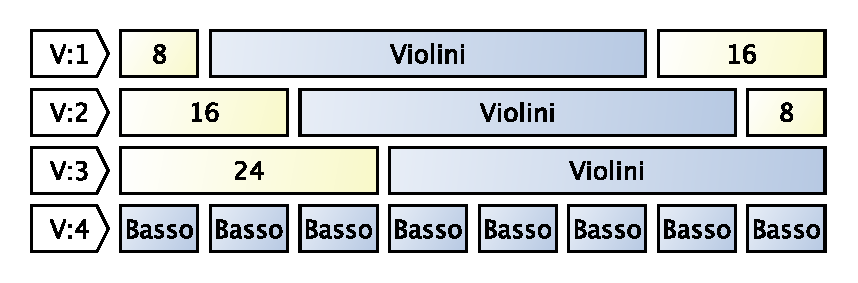
\includegraphics[width=0.8\textwidth]{img/pcanon_scheme.pdf}
    \caption{\canonabc{}'s output scheme}
    \label{fig:pcanon_scheme}
  \end{center}
\end{figure}


\section{Working Together}
This section shows a real example of how to combine three of the \abcpt{}s created: \catabc{},
\pasteabc{} and \learningabc{}.

In this example, a user wants to study his voice (\emph{Tenor}) and \emph{Soprano}'s on the first three sections
of the \emph{Christmas Villancico}\footnote{A Villancico is a musical and poetic form written in
Spanish and Portuguese, traditional from Spain, Latin America and Portugal. These pieces were
popular between century XV and XVIII.} \textit{Verbum caro factum est}.

Each section and voice is written in separate files, so the parts requested will be assembled by
combining \pasteabc{} with \catabc{}.

Then \learningabc{} is going to be used with the combined score in order to produce two scores: one
where voice \emph{Tenor} is highlighted and another where the other voices are.

Listing \ref{lst:cat_paste_by_example} shows the first step being put into action. Listing
\ref{lst:verbum} shows its output, which, in this section, is going to be referred to as
\emph{verbum.abc} and figure \ref{fig:verbum} the corresponding score.\\

\begin{lstlisting}[caption={\catabc{} and \pasteabc{} by example},label={lst:cat_paste_by_example},captionpos=t,abovecaptionskip=-\medskipamount]
cat_abc (
  paste_abc ( 101.abc 103.abc )
  cat_abc   ( 201.abc 303.abc )
) > verbum.abc
\end{lstlisting}

\vspace{1cm}
\lstinputlisting[caption={\emph{verbum.abc}},label={lst:verbum},captionpos=t,abovecaptionskip=-\medskipamount]{misc/verbum.tex}

% \vspace{-1.30cm}
\begin{figure}[H]
  \centering
  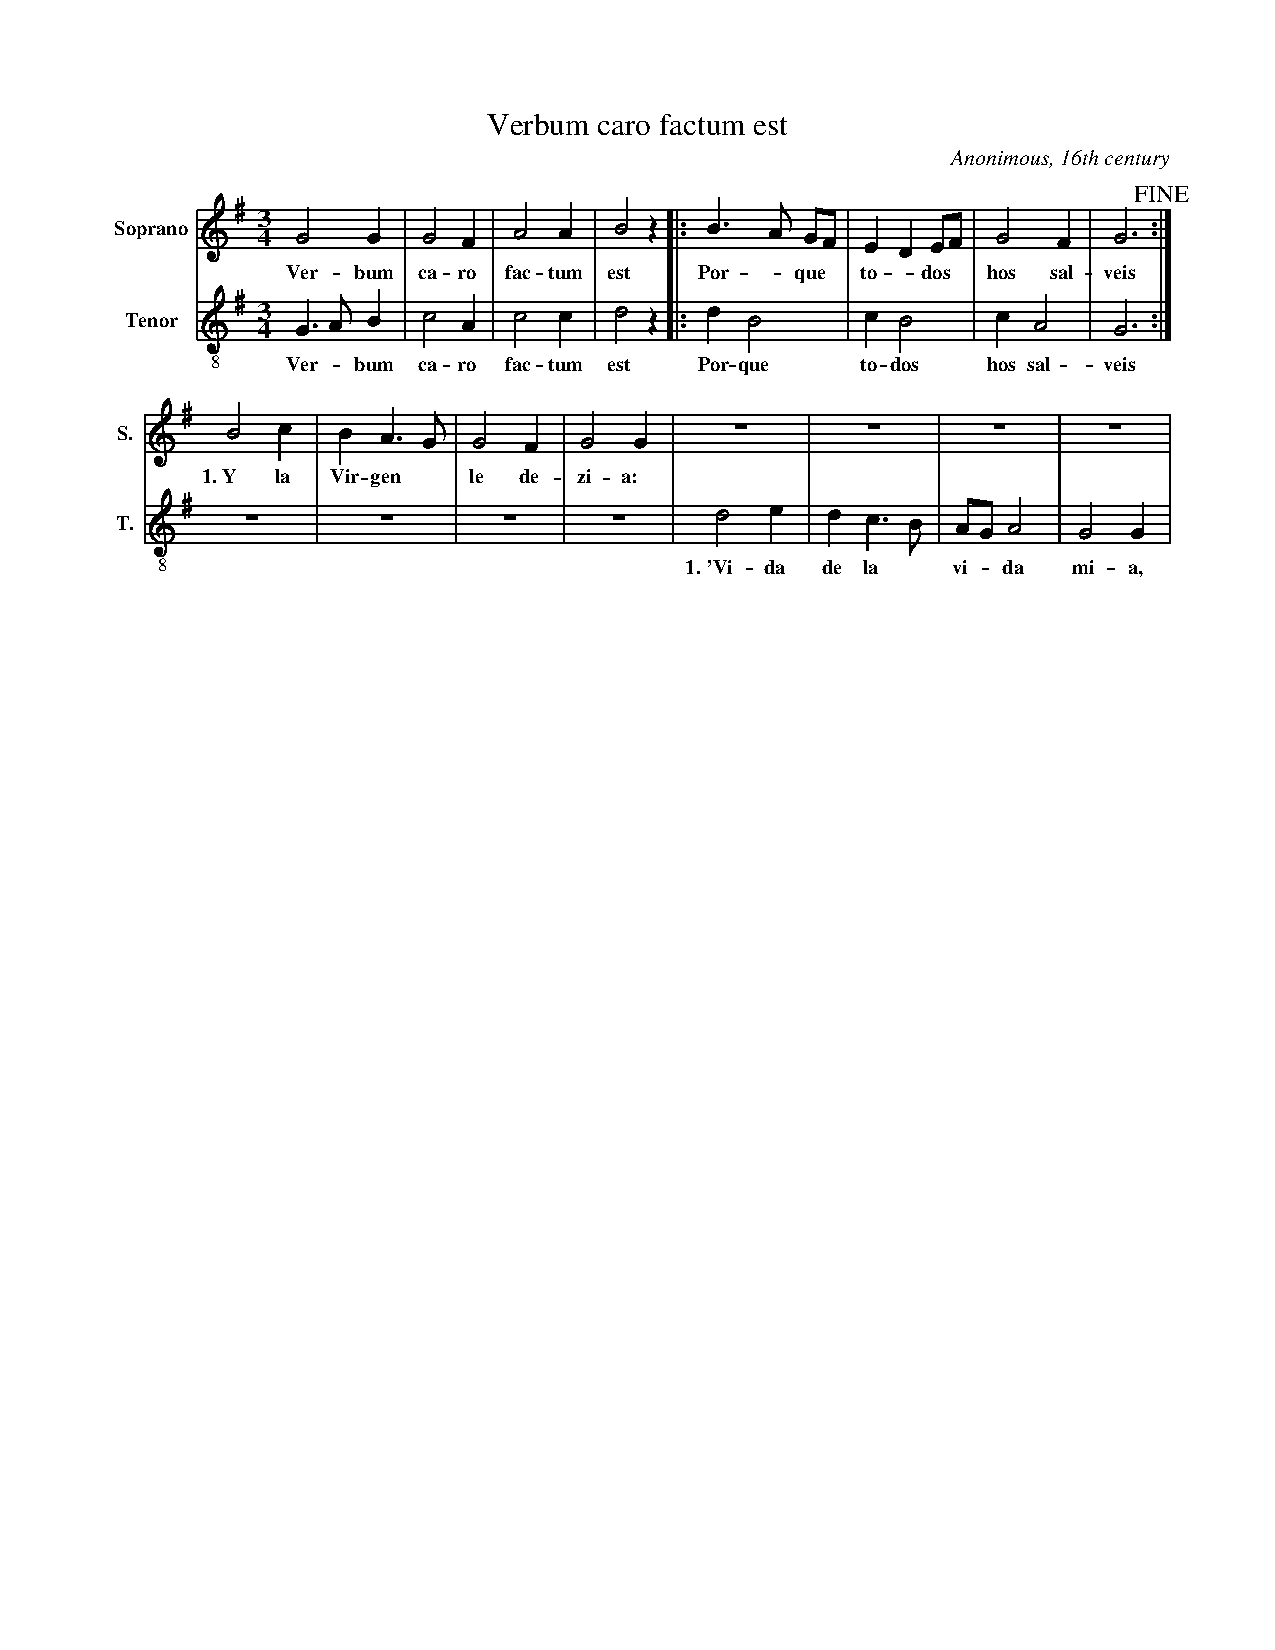
\includegraphics[width=0.8\textwidth, clip=true, trim = 15mm 180mm 15mm 30mm]{img/verbum.pdf}
  \caption{Verbum caro factum est Score: Sections 1, 2 \& 3; Parts 1 \& 3}
  \label{fig:verbum}
\end{figure}

After putting the score together, it's time to modify it in order to help the user study. So
\learningabc{} (see listing \ref{lst:learning_on_cat_paste}) generates a score where just voice
\emph{Tenor} is highlighted (\ref{lst:just_tenor}) and one where all voices but \emph{Tenor}'s are
highlighted (\ref{lst:all_but_tenor}).\\

\begin{lstlisting}[caption={\learningabc{} on combined score},label={lst:learning_on_cat_paste},captionpos=t,abovecaptionskip=-\medskipamount]
learning_abc -v=Tenor verbum.abc
\end{lstlisting}

\lstinputlisting[caption={verbum\_just\_Tenor.abc},label={lst:just_tenor},captionpos=t,abovecaptionskip=-\medskipamount]{misc/v_just_Tenor.tex}
\lstinputlisting[caption={verbum\_all\_but\_Tenor.abc},label={lst:all_but_tenor},captionpos=t,abovecaptionskip=-\medskipamount]{misc/v_all_but_Tenor.tex}

